% !Mode:: "TeX:UTF-8"

\chapter[贪心算法并行化]{贪心算法并行化}
\section{贪心算法介绍}
    贪心算法的核心思想是每次局部决策时选择当前最优的解,以期待能够获得最优的全局解。很多问题虽然贪心算法并不能获得
一个全局的解法,但是贪心算法能够在较短时间内得到近似于全局最优解. 

    通常来说,一个贪心算法包含了5个组件:

    \begin{itemize}
        \item 候选集,即问题集
        \item 选择函数,将当前最佳的问题解添加到全局解
        \item 可行性函数,用来决定候选解是否是当前最佳的问题解
        \item 目标函数,用来获取局部最优解
        \item 解决函数,用来知识全部的最优解
    \end{itemize}

    本文以Dijkstra最短路径算法为例子。随着计算机处理数据量增多,串行计算机的计算量已经无法满足现代大数据量的计算
要求,只有基于并行算法的最短路径算法才能在大量的数据中实时或者接近实时的方式,使用计算机的计算和存储能力来获取足够快
的结果.Dijkstra提出了按路径长度不减次序产生的最短路径的算法,假设, 给定带权有向图G =(V,E),
其中每条边的权是非负实数。另外,还给定V中的一个顶点,称为源。现在要计算从源到所有其它各顶点的最短路长度。这里路的长度是指路上各边权之和。这个问题通常称为单源最短路径问题。
Dijkstra算法是解决有向图中单个源点到其他顶点的最短路径问题的贪心算法。

    并行的Dijkstra算法目标是将所有数据计算节点进行合理划分,实现计算平衡,将类似的子问题划分到不同的处理器上,各个
处理器进行子问题计算,最后汇聚全部处理器的解,从而得到最优解.

\section{算法描述}
    
    Dijkstra算法的输入包含了一个有权重的有向图G,以及G中的一个来源顶点S。我们以V表示G中所有顶点的集合。每一个图中的边,都
是两个顶点所形成的有序元素对。(u,v) 表示从顶点u到v有路径相连。我们以E所有边的集合,而边的权重则由权重函数$w: E \rightarrow [0, \infty]$
定义。因此,w(u, v) 就是从顶点u到顶点v的非负权重(weight)。边的权重可以想像成两个顶点之间的距离。任两点间路径的权重,就
是该路径上所有边的权重总和。已知有 V 中有顶点 s 及 t.Dijkstra算法可以找到s到t的最低权重路径(例如,最短路径)。这个算法也
可以在一个图中,找到从一个顶点 s 到任何其他顶点的最短路径。

    这个算法是通过为每个顶点 v 保留目前为止所找到的从s到v的最短路径来工作的。初始时,原点 s 的路径长度值被赋为 0 (d[s] = 0),
若存在能直接到达的边(s,m),则把d[m]设为w(s,m),同时把所有其他(s不能直接到达的)顶点的路径长度设为无穷大,即表示我们不知道
任何通向这些顶点的路径(对于 V 中所有顶点 v 除 s 和上述 m 外$ d[v] =\infty $)。当算法退出时,d[v] 中存储的便是从s到v的最短路径,
或者如果路径不存在的话是无穷大。 

    Dijkstra 算法的基础操作是边的拓展:如果存在一条从u到v的边,那么从s到v的最短路径可以通过将边(u, v)添加到尾部来拓展一条从
s到u的路径。这条路径的长度是d[u]+ w(u, v)。如果这个值比目前已知的 d[v] 的值要小,我们可以用新值来替代当前d[v]中的值。
拓展边的操作一直运行到所有的d[v]都代表从s到v最短路径的花费。这个算法经过组织因而当d[u]达到它最终的值的时候每条边(u, v)
都只被拓展一次。 

算法维护两个顶点集S和Q。集合S保留了我们已知的所有d[v]的值已经是最短路径的值顶点,而集合 Q 则保留其他所有顶点。集合S初始状态为空,
而后每一步都有一个顶点从Q移动到S。这个被选择的顶点是Q中拥有最小的d[u]值的顶点。当一个顶点u从Q中转移到了S中,算法对每条外接边 (u, v)
进行拓展。
\\
    算法流程图,如图~\ref{fig:dijkstra}所示

    \begin{figure}[htbp]
    \centering
    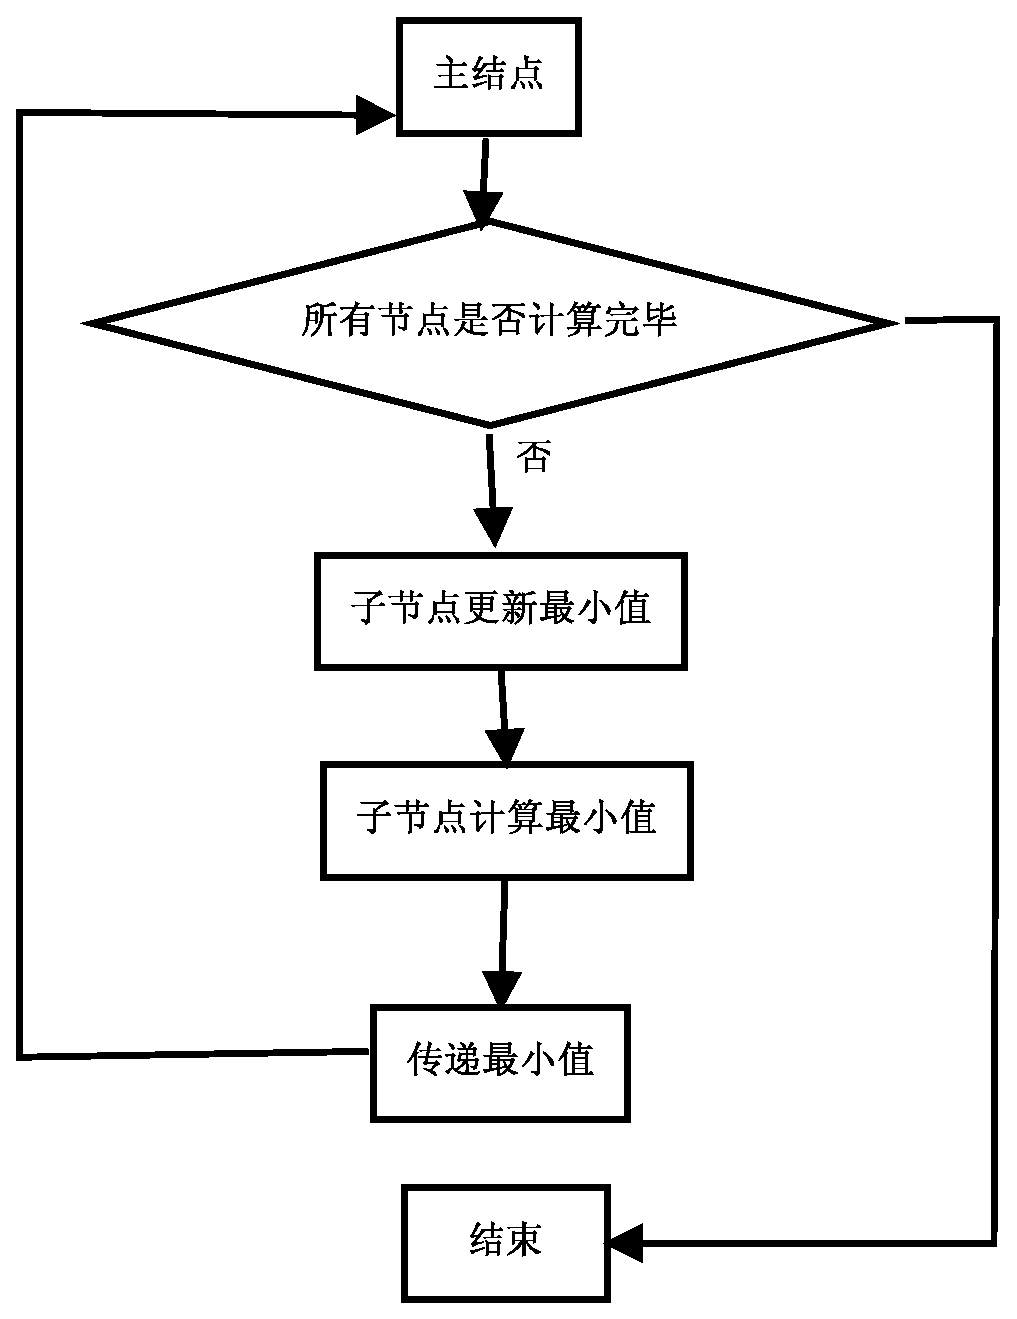
\includegraphics[width=0.6\textwidth]{dijkstra}
    \caption{dijkstra}\label{fig:dijkstra}
    \vspace{\baselineskip}
    \end{figure}

    Dijkstra并行最短路径搜索算法的算法步骤:
    \begin{enumerate}
    \item 将问题进行结点划分,每个处理器分配$n=\frac{N}{P}$其中N表示结点总数,P表示节点数目
    \item 每个处理器并行计算局部的最小值,主节点收集所有的局部最小值,并获取所有局部最小值中的最小值,得到全局最小值
            $Global_{min}$,标记该最小值的位置index,广播$Global_{min}$和index至所有的结点
    \item 每个处理器获取全局最小之后进行更新,if($Global_{min}$+W(v,index)<dist(v)) update(dist(v)=min+W(v,index))
    \item 重复第2,和第3步,直到目标结点被标记为止
    \end{enumerate}
            
\section{算法伪代码}

\begin{algorithmic}
\State $Done = {0}$
\State $NonDone = {1,2,\ldots,N-1}$
\State $MPI\_Barrier(MPI\_COMM\_WORLD)$
\For {$J \gets 1 to N-1 $} \State $Dist[j]=infinity$ \EndFor
\State $Dist[0]=0$
\For {$Step = 1  to myrank $}
    \State find J such that Dist[j] is min among all J in NonDone
    \State transfer J from NonDone to Done
    \State $NewDone = J$
    \For {$K=1 to myrank$}
        \If {K is in NonDone}
            \State Dist[k] = min(Dist[k],Dist[NewDone]+G[NewDone,k])
        \EndIf
    \EndFor
\EndFor
\If{$myrank=0$}
\State ${MPI\_Gather(Dist[k],node,MPI\_DOUBLE,allmin,node,MPI\_DOUBLE,MPI\_COMM\_WORLD)} $
\EndIf
\For{$i=0;i < p;i++$}
\State $allmin=Global_{min}$
\EndFor
\State $MPI\_Bcast(min0,1,MPI\_DOUBLE,1,MPI\_COMM\_WORLD);$


\end{algorithmic}

\section{实验结果}
\subsection{加速比}
    传统算法的时间复杂度为$O(N^2)$,并行算法的时间复杂度为$O(\frac{N^2}{p}+N*(p-1))$,其中每次并行计算时
需要对每一个全局最小值进行p个局部最小值的比较,共需要N次比较.所以并行化的加速比为
    $$S=\frac{O(N^2)}{O(\frac{N^2}{p}+N*(p-1))}$$
\subsection{实验结果分析}
    本次试验结果通过MPI自带的MPI\_Wtime{}来统计程序的运行时间,分别采用单机和分布式的方式来统计程序
运行的时间和效率,每次时间通过多次实验去平均值的方法,每个结点采取多次计算的方式.
    \begin{table}[htbp]
    \centering  % 表居中
    \begin{tabular}{lcc}  % {lccc} 表示各列元素对齐方式,left-l,right-r,center-c
    \hline
    节点数&单机&并行\\ \hline  % \hline 在此行下面画一横线
    200&1.649&0.530 \\
    400&3.043&0.792 \\
    600&5.189&1.424 \\
    800&7.198&1.952 \\
    1000&8.325&2.362 \\
    1200&9.889&2.626 \\
    1400&11.327&3.277 \\ \hline
    \end{tabular}
    \caption{算法时间对比总结}
    \end{table}

当节点数目不多时,MPI的算法呈直线增长,但是当节点数目增加时,由于进程间通信消耗时间增多,导致增长
速度缓慢,而单机串行算法始终保持一种线性关系的增长,

%    加速比图

%%%http://zh.wikipedia.org/zh-cn/%E8%BF%AA%E7%A7%91%E6%96%AF%E5%BD%BB%E7%AE%97%E6%B3%95
%http://en.wikipedia.org/wiki/Dijkstra%27s_algorithm
%http://heather.cs.ucdavis.edu/~matloff/145/ParScript/MPI.pdf
%http://heather.cs.ucdavis.edu/~matloff/145/ParScript/MPI.pdf
